\documentclass[a4paper]{scrartcl}

% UTF-8 encoding
\usepackage[utf8]{inputenc}

\usepackage{graphicx}

% Meta informations
\title{5 Stereo matching with dynamic programming}
\subtitle{Computer Vision practical seminar \\ TU Dresden}
\author{Lucas Kahlert}
\date{\today}

\begin{document}

\maketitle

\section{Stereo matching with dynamic programming}

There was multiple matchings started for the different parameter sets.
The results and parameters are given in the next subsections.

If no other parameter is given, the following defaults are used:

\begin{table}
  \begin{tabular}{ l l l }
    window-size   : &  5 px \\
    max disparity : &  15 px \\
    scale-cost    : &  0.075 & // weight of cost function \\
    cost-function : &  absolute difference \\
    topology      : &  line & // all rows connected via a line in the middle) \\
  \end{tabular}
  \caption{Default parameters}
\end{table}


\section{Different parameters}

\subsection{Topology}

The tree have little influence on the streaking effect occuring
with chains. The reason for this is the weak topology of the
spanning tree, which consits nearly completly of chains.

\vspace{1cm}
\begin{minipage}{0.8\textwidth}
  \centering
  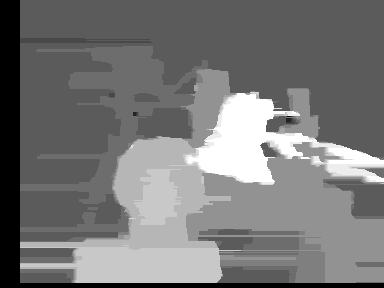
\includegraphics[width=0.8\textwidth]{images/line.png}
  \captionof{figure}{Markov chain with streaking effect}
\end{minipage}

\vspace{1cm}
\begin{minipage}{0.8\textwidth}
  \centering
  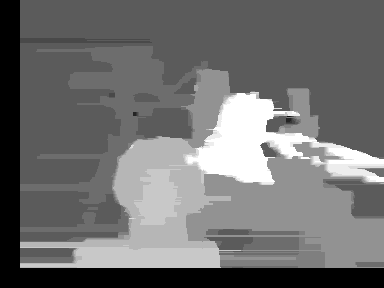
\includegraphics[width=0.8\textwidth]{images/defaults.png}
  \captionof{figure}{Default parameters on a tree}
\end{minipage}


\subsection{Window size}

A larger windows size for the matching of two patches results in
a coarser disparity map.

\vspace{1cm}
\begin{minipage}{0.8\textwidth}
  \centering
  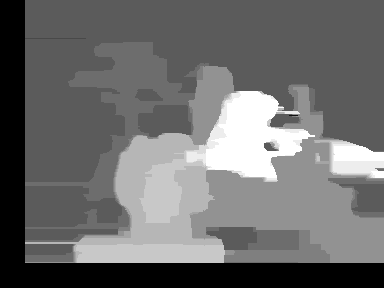
\includegraphics[width=0.8\textwidth]{images/window_size-10.png}
  \captionof{figure}{Window size of 10px}
\end{minipage}

\vspace{1cm}
\begin{minipage}{0.8\textwidth}
  \centering
  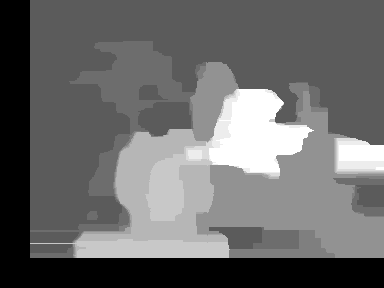
\includegraphics[width=0.8\textwidth]{images/window_size-15.png}
  \captionof{figure}{Window size of 15px}
\end{minipage}


\subsection{Cost functions}

A cost function that gives a higher penalty for larger differences
returns better results than a simple delta function (Potts model).

\vspace{1cm}
\begin{minipage}{0.8\textwidth}
  \centering
  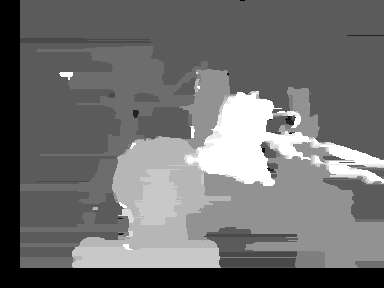
\includegraphics[width=0.8\textwidth]{images/potts.png}
  \captionof{figure}{Potts model}
\end{minipage}

\vspace{1cm}
\begin{minipage}{0.8\textwidth}
  \centering
  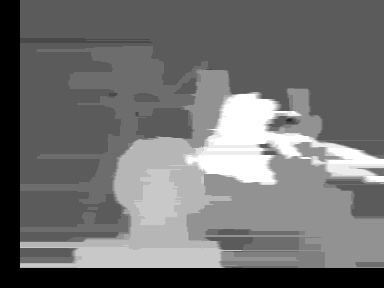
\includegraphics[width=0.8\textwidth]{images/squarediff.png}
  \captionof{figure}{Square difference as cost function}
\end{minipage}


\subsection{Scaling factor}

For higher scaling factor for the costs, we got more homogenous
areas of disparity.

\vspace{1cm}
\begin{minipage}{0.8\textwidth}
  \centering
  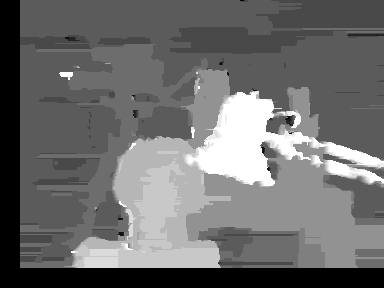
\includegraphics[width=0.8\textwidth]{images/scale-0.005.png}
  \captionof{figure}{Scaling factor 0.005}
\end{minipage}

\vspace{1cm}
\begin{minipage}{0.8\textwidth}
  \centering
  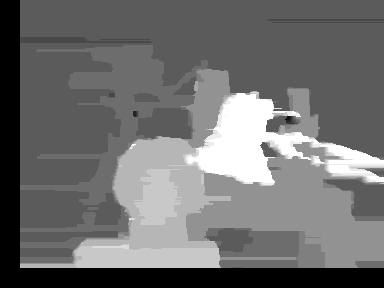
\includegraphics[width=0.8\textwidth]{images/scale-0.05.png}
  \captionof{figure}{Scaling factor 0.05}
\end{minipage}

\vspace{1cm}
\begin{minipage}{0.8\textwidth}
  \centering
  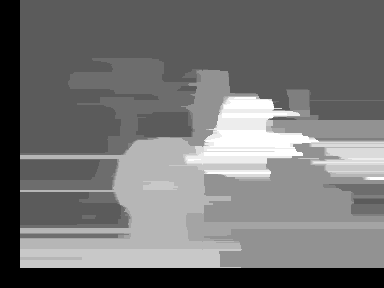
\includegraphics[width=0.8\textwidth]{images/scale-0.5.png}
  \captionof{figure}{Scaling factor 0.5}
\end{minipage}


\end{document}
